\documentclass[twoside]{book}

% Packages required by doxygen
\usepackage{fixltx2e}
\usepackage{calc}
\usepackage{doxygen}
\usepackage[export]{adjustbox} % also loads graphicx
\usepackage{graphicx}
\usepackage[utf8]{inputenc}
\usepackage{makeidx}
\usepackage{multicol}
\usepackage{multirow}
\PassOptionsToPackage{warn}{textcomp}
\usepackage{textcomp}
\usepackage[nointegrals]{wasysym}
\usepackage[table]{xcolor}

% Font selection
\usepackage[T1]{fontenc}
\usepackage[scaled=.90]{helvet}
\usepackage{courier}
\usepackage{amssymb}
\usepackage{sectsty}
\renewcommand{\familydefault}{\sfdefault}
\allsectionsfont{%
  \fontseries{bc}\selectfont%
  \color{darkgray}%
}
\renewcommand{\DoxyLabelFont}{%
  \fontseries{bc}\selectfont%
  \color{darkgray}%
}
\newcommand{\+}{\discretionary{\mbox{\scriptsize$\hookleftarrow$}}{}{}}

% Page & text layout
\usepackage{geometry}
\geometry{%
  a4paper,%
  top=2.5cm,%
  bottom=2.5cm,%
  left=2.5cm,%
  right=2.5cm%
}
\tolerance=750
\hfuzz=15pt
\hbadness=750
\setlength{\emergencystretch}{15pt}
\setlength{\parindent}{0cm}
\setlength{\parskip}{3ex plus 2ex minus 2ex}
\makeatletter
\renewcommand{\paragraph}{%
  \@startsection{paragraph}{4}{0ex}{-1.0ex}{1.0ex}{%
    \normalfont\normalsize\bfseries\SS@parafont%
  }%
}
\renewcommand{\subparagraph}{%
  \@startsection{subparagraph}{5}{0ex}{-1.0ex}{1.0ex}{%
    \normalfont\normalsize\bfseries\SS@subparafont%
  }%
}
\makeatother

% Headers & footers
\usepackage{fancyhdr}
\pagestyle{fancyplain}
\fancyhead[LE]{\fancyplain{}{\bfseries\thepage}}
\fancyhead[CE]{\fancyplain{}{}}
\fancyhead[RE]{\fancyplain{}{\bfseries\leftmark}}
\fancyhead[LO]{\fancyplain{}{\bfseries\rightmark}}
\fancyhead[CO]{\fancyplain{}{}}
\fancyhead[RO]{\fancyplain{}{\bfseries\thepage}}
\fancyfoot[LE]{\fancyplain{}{}}
\fancyfoot[CE]{\fancyplain{}{}}
\fancyfoot[RE]{\fancyplain{}{\bfseries\scriptsize Generated by Doxygen }}
\fancyfoot[LO]{\fancyplain{}{\bfseries\scriptsize Generated by Doxygen }}
\fancyfoot[CO]{\fancyplain{}{}}
\fancyfoot[RO]{\fancyplain{}{}}
\renewcommand{\footrulewidth}{0.4pt}
\renewcommand{\chaptermark}[1]{%
  \markboth{#1}{}%
}
\renewcommand{\sectionmark}[1]{%
  \markright{\thesection\ #1}%
}

% Indices & bibliography
\usepackage{natbib}
\usepackage[titles]{tocloft}
\setcounter{tocdepth}{3}
\setcounter{secnumdepth}{5}
\makeindex

% Hyperlinks (required, but should be loaded last)
\usepackage{ifpdf}
\ifpdf
  \usepackage[pdftex,pagebackref=true]{hyperref}
\else
  \usepackage[ps2pdf,pagebackref=true]{hyperref}
\fi
\hypersetup{%
  colorlinks=true,%
  linkcolor=blue,%
  citecolor=blue,%
  unicode%
}

% Custom commands
\newcommand{\clearemptydoublepage}{%
  \newpage{\pagestyle{empty}\cleardoublepage}%
}

\usepackage{caption}
\captionsetup{labelsep=space,justification=centering,font={bf},singlelinecheck=off,skip=4pt,position=top}

%===== C O N T E N T S =====

\begin{document}

% Titlepage & ToC
\hypersetup{pageanchor=false,
             bookmarksnumbered=true,
             pdfencoding=unicode
            }
\pagenumbering{roman}
\begin{titlepage}
\vspace*{7cm}
\begin{center}%
{\Large My Project }\\
\vspace*{1cm}
{\large Generated by Doxygen 1.8.11}\\
\end{center}
\end{titlepage}
\clearemptydoublepage
\tableofcontents
\clearemptydoublepage
\pagenumbering{arabic}
\hypersetup{pageanchor=true}

%--- Begin generated contents ---
\chapter{Hierarchical Index}
\section{Class Hierarchy}
This inheritance list is sorted roughly, but not completely, alphabetically\+:\begin{DoxyCompactList}
\item \contentsline{section}{Fruit}{\pageref{classFruit}}{}
\begin{DoxyCompactList}
\item \contentsline{section}{Apple}{\pageref{classApple}}{}
\item \contentsline{section}{Grape}{\pageref{classGrape}}{}
\item \contentsline{section}{Orange}{\pageref{classOrange}}{}
\end{DoxyCompactList}
\item \contentsline{section}{List}{\pageref{classList}}{}
\item \contentsline{section}{List\+:\+:Node}{\pageref{structList_1_1Node}}{}
\end{DoxyCompactList}

\chapter{Class Index}
\section{Class List}
Here are the classes, structs, unions and interfaces with brief descriptions\+:\begin{DoxyCompactList}
\item\contentsline{section}{\hyperlink{structnode}{node} }{\pageref{structnode}}{}
\item\contentsline{section}{\hyperlink{structnode1}{node1} }{\pageref{structnode1}}{}
\item\contentsline{section}{\hyperlink{structnode__info}{node\+\_\+info} }{\pageref{structnode__info}}{}
\end{DoxyCompactList}

\chapter{File Index}
\section{File List}
Here is a list of all files with brief descriptions\+:\begin{DoxyCompactList}
\item\contentsline{section}{\hyperlink{Lab1_8c}{Lab1.\+c} }{\pageref{Lab1_8c}}{}
\end{DoxyCompactList}

\chapter{Class Documentation}
\hypertarget{classApple}{}\section{Apple Class Reference}
\label{classApple}\index{Apple@{Apple}}


Inheritance diagram for Apple\+:
\nopagebreak
\begin{figure}[H]
\begin{center}
\leavevmode
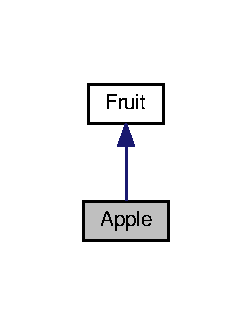
\includegraphics[width=121pt]{classApple__inherit__graph}
\end{center}
\end{figure}


Collaboration diagram for Apple\+:
\nopagebreak
\begin{figure}[H]
\begin{center}
\leavevmode
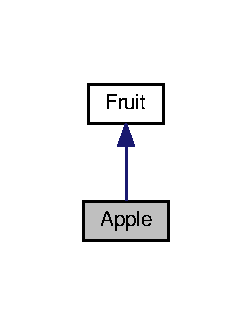
\includegraphics[width=121pt]{classApple__coll__graph}
\end{center}
\end{figure}
\subsection*{Public Member Functions}
\begin{DoxyCompactItemize}
\item 
\hyperlink{classApple_ac294391728d8503a83eccc8be50667bf}{Apple} (string name)
\item 
virtual void \hyperlink{classApple_a6397c19d951c6e0e158f56eac34a25ec}{print} () const 
\end{DoxyCompactItemize}
\subsection*{Additional Inherited Members}


\subsection{Constructor \& Destructor Documentation}
\index{Apple@{Apple}!Apple@{Apple}}
\index{Apple@{Apple}!Apple@{Apple}}
\subsubsection[{\texorpdfstring{Apple(string name)}{Apple(string name)}}]{\setlength{\rightskip}{0pt plus 5cm}Apple\+::\+Apple (
\begin{DoxyParamCaption}
\item[{string}]{name}
\end{DoxyParamCaption}
)\hspace{0.3cm}{\ttfamily [inline]}}\hypertarget{classApple_ac294391728d8503a83eccc8be50667bf}{}\label{classApple_ac294391728d8503a83eccc8be50667bf}

\begin{DoxyCode}
26 : \hyperlink{classFruit_ad5e1cedbbe3153aad5b66533f9664e64}{Fruit}(name) \{\}
\end{DoxyCode}


\subsection{Member Function Documentation}
\index{Apple@{Apple}!print@{print}}
\index{print@{print}!Apple@{Apple}}
\subsubsection[{\texorpdfstring{print() const }{print() const }}]{\setlength{\rightskip}{0pt plus 5cm}virtual void Apple\+::print (
\begin{DoxyParamCaption}
{}
\end{DoxyParamCaption}
) const\hspace{0.3cm}{\ttfamily [inline]}, {\ttfamily [virtual]}}\hypertarget{classApple_a6397c19d951c6e0e158f56eac34a25ec}{}\label{classApple_a6397c19d951c6e0e158f56eac34a25ec}


Implements \hyperlink{classFruit_aa939d4077d9be227dde4e8649649c5a2}{Fruit}.


\begin{DoxyCode}
27 \{ cout << \hyperlink{classFruit_a97df614e17aebaae352e97d51c801906}{owner} << \textcolor{stringliteral}{"'s apple"} << endl; \}
\end{DoxyCode}


The documentation for this class was generated from the following file\+:\begin{DoxyCompactItemize}
\item 
\hyperlink{Fruit_8cpp}{Fruit.\+cpp}\end{DoxyCompactItemize}

\hypertarget{classFruit}{}\section{Fruit Class Reference}
\label{classFruit}\index{Fruit@{Fruit}}


Inheritance diagram for Fruit\+:
\nopagebreak
\begin{figure}[H]
\begin{center}
\leavevmode
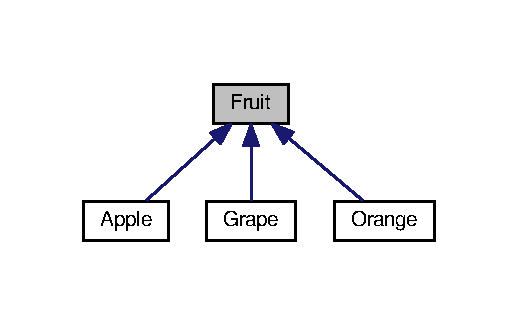
\includegraphics[width=249pt]{classFruit__inherit__graph}
\end{center}
\end{figure}
\subsection*{Public Member Functions}
\begin{DoxyCompactItemize}
\item 
\hyperlink{classFruit_ad5e1cedbbe3153aad5b66533f9664e64}{Fruit} (string name)
\item 
virtual void \hyperlink{classFruit_aa939d4077d9be227dde4e8649649c5a2}{print} () const =0
\end{DoxyCompactItemize}
\subsection*{Protected Attributes}
\begin{DoxyCompactItemize}
\item 
string \hyperlink{classFruit_a97df614e17aebaae352e97d51c801906}{owner}
\end{DoxyCompactItemize}


\subsection{Constructor \& Destructor Documentation}
\index{Fruit@{Fruit}!Fruit@{Fruit}}
\index{Fruit@{Fruit}!Fruit@{Fruit}}
\subsubsection[{\texorpdfstring{Fruit(string name)}{Fruit(string name)}}]{\setlength{\rightskip}{0pt plus 5cm}Fruit\+::\+Fruit (
\begin{DoxyParamCaption}
\item[{string}]{name}
\end{DoxyParamCaption}
)\hspace{0.3cm}{\ttfamily [inline]}}\hypertarget{classFruit_ad5e1cedbbe3153aad5b66533f9664e64}{}\label{classFruit_ad5e1cedbbe3153aad5b66533f9664e64}

\begin{DoxyCode}
18 \{ \hyperlink{classFruit_a97df614e17aebaae352e97d51c801906}{owner} = name; \}
\end{DoxyCode}


\subsection{Member Function Documentation}
\index{Fruit@{Fruit}!print@{print}}
\index{print@{print}!Fruit@{Fruit}}
\subsubsection[{\texorpdfstring{print() const =0}{print() const =0}}]{\setlength{\rightskip}{0pt plus 5cm}virtual void Fruit\+::print (
\begin{DoxyParamCaption}
{}
\end{DoxyParamCaption}
) const\hspace{0.3cm}{\ttfamily [pure virtual]}}\hypertarget{classFruit_aa939d4077d9be227dde4e8649649c5a2}{}\label{classFruit_aa939d4077d9be227dde4e8649649c5a2}


Implemented in \hyperlink{classGrape_a15be78acef26a255c161cbe7c6d7ed1b}{Grape}, \hyperlink{classOrange_acb75bbb15104ce63afa0cc6712e239e4}{Orange}, and \hyperlink{classApple_a6397c19d951c6e0e158f56eac34a25ec}{Apple}.



\subsection{Member Data Documentation}
\index{Fruit@{Fruit}!owner@{owner}}
\index{owner@{owner}!Fruit@{Fruit}}
\subsubsection[{\texorpdfstring{owner}{owner}}]{\setlength{\rightskip}{0pt plus 5cm}string Fruit\+::owner\hspace{0.3cm}{\ttfamily [protected]}}\hypertarget{classFruit_a97df614e17aebaae352e97d51c801906}{}\label{classFruit_a97df614e17aebaae352e97d51c801906}


The documentation for this class was generated from the following file\+:\begin{DoxyCompactItemize}
\item 
\hyperlink{Fruit_8cpp}{Fruit.\+cpp}\end{DoxyCompactItemize}

\hypertarget{classGrape}{}\section{Grape Class Reference}
\label{classGrape}\index{Grape@{Grape}}


Inheritance diagram for Grape\+:
\nopagebreak
\begin{figure}[H]
\begin{center}
\leavevmode
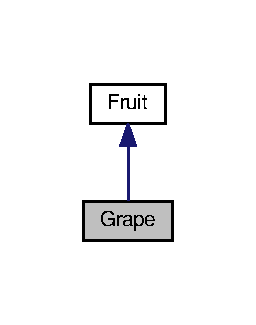
\includegraphics[width=123pt]{classGrape__inherit__graph}
\end{center}
\end{figure}


Collaboration diagram for Grape\+:
\nopagebreak
\begin{figure}[H]
\begin{center}
\leavevmode
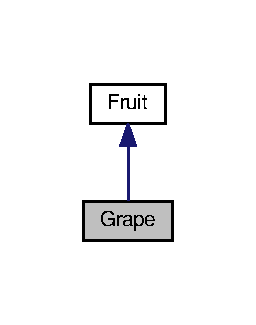
\includegraphics[width=123pt]{classGrape__coll__graph}
\end{center}
\end{figure}
\subsection*{Public Member Functions}
\begin{DoxyCompactItemize}
\item 
\hyperlink{classGrape_ad6a21e427a3605149a54555d6c026f2c}{Grape} (string name)
\item 
virtual void \hyperlink{classGrape_a15be78acef26a255c161cbe7c6d7ed1b}{print} () const 
\end{DoxyCompactItemize}
\subsection*{Additional Inherited Members}


\subsection{Constructor \& Destructor Documentation}
\index{Grape@{Grape}!Grape@{Grape}}
\index{Grape@{Grape}!Grape@{Grape}}
\subsubsection[{\texorpdfstring{Grape(string name)}{Grape(string name)}}]{\setlength{\rightskip}{0pt plus 5cm}Grape\+::\+Grape (
\begin{DoxyParamCaption}
\item[{string}]{name}
\end{DoxyParamCaption}
)\hspace{0.3cm}{\ttfamily [inline]}}\hypertarget{classGrape_ad6a21e427a3605149a54555d6c026f2c}{}\label{classGrape_ad6a21e427a3605149a54555d6c026f2c}

\begin{DoxyCode}
44 : \hyperlink{classFruit_ad5e1cedbbe3153aad5b66533f9664e64}{Fruit}(name) \{\}
\end{DoxyCode}


\subsection{Member Function Documentation}
\index{Grape@{Grape}!print@{print}}
\index{print@{print}!Grape@{Grape}}
\subsubsection[{\texorpdfstring{print() const }{print() const }}]{\setlength{\rightskip}{0pt plus 5cm}virtual void Grape\+::print (
\begin{DoxyParamCaption}
{}
\end{DoxyParamCaption}
) const\hspace{0.3cm}{\ttfamily [inline]}, {\ttfamily [virtual]}}\hypertarget{classGrape_a15be78acef26a255c161cbe7c6d7ed1b}{}\label{classGrape_a15be78acef26a255c161cbe7c6d7ed1b}


Implements \hyperlink{classFruit_aa939d4077d9be227dde4e8649649c5a2}{Fruit}.


\begin{DoxyCode}
45 \{ cout << \hyperlink{classFruit_a97df614e17aebaae352e97d51c801906}{owner} << \textcolor{stringliteral}{"'s grape"} << endl; \}
\end{DoxyCode}


The documentation for this class was generated from the following file\+:\begin{DoxyCompactItemize}
\item 
\hyperlink{Fruit_8cpp}{Fruit.\+cpp}\end{DoxyCompactItemize}

\hypertarget{classList}{}\section{List Class Reference}
\label{classList}\index{List@{List}}


Collaboration diagram for List\+:
\nopagebreak
\begin{figure}[H]
\begin{center}
\leavevmode
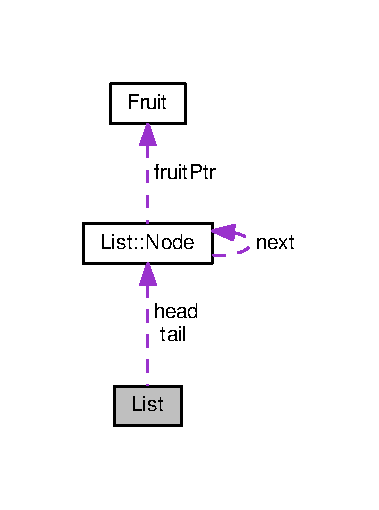
\includegraphics[width=182pt]{classList__coll__graph}
\end{center}
\end{figure}
\subsection*{Classes}
\begin{DoxyCompactItemize}
\item 
struct \hyperlink{structList_1_1Node}{Node}
\end{DoxyCompactItemize}
\subsection*{Public Member Functions}
\begin{DoxyCompactItemize}
\item 
\hyperlink{classList_a06e2fd0daed0264a70fb70194e7d93b6}{List} (\hyperlink{classFruit}{Fruit} $\ast$a\+Fruit)
\item 
\hyperlink{classList_a70aecf37bd9d779a394e4d50377fbf5f}{$\sim$\+List} ()
\item 
void \hyperlink{classList_aa38578a39e87e4b5d349d50e179dfa7a}{append} (\hyperlink{classFruit}{Fruit} $\ast$a\+Fruit)
\item 
void \hyperlink{classList_a1bb66c2777061ab3b8260746a8c3961e}{print\+List} ()
\end{DoxyCompactItemize}
\subsection*{Private Attributes}
\begin{DoxyCompactItemize}
\item 
\hyperlink{structList_1_1Node}{Node} $\ast$ \hyperlink{classList_a443db628080a04a1dacfd3015d164735}{head}
\item 
\hyperlink{structList_1_1Node}{Node} $\ast$ \hyperlink{classList_ac35bbbb4a3103f9574e74491d52dbeba}{tail}
\end{DoxyCompactItemize}


\subsection{Constructor \& Destructor Documentation}
\index{List@{List}!List@{List}}
\index{List@{List}!List@{List}}
\subsubsection[{\texorpdfstring{List(\+Fruit $\ast$a\+Fruit)}{List(Fruit *aFruit)}}]{\setlength{\rightskip}{0pt plus 5cm}List\+::\+List (
\begin{DoxyParamCaption}
\item[{{\bf Fruit} $\ast$}]{a\+Fruit}
\end{DoxyParamCaption}
)\hspace{0.3cm}{\ttfamily [inline]}}\hypertarget{classList_a06e2fd0daed0264a70fb70194e7d93b6}{}\label{classList_a06e2fd0daed0264a70fb70194e7d93b6}

\begin{DoxyCode}
59 \{\hyperlink{classList_a443db628080a04a1dacfd3015d164735}{head} = \hyperlink{classList_ac35bbbb4a3103f9574e74491d52dbeba}{tail} = \textcolor{keyword}{new} Node(aFruit); \}
\end{DoxyCode}
\index{List@{List}!````~List@{$\sim$\+List}}
\index{````~List@{$\sim$\+List}!List@{List}}
\subsubsection[{\texorpdfstring{$\sim$\+List()}{~List()}}]{\setlength{\rightskip}{0pt plus 5cm}List\+::$\sim$\+List (
\begin{DoxyParamCaption}
{}
\end{DoxyParamCaption}
)\hspace{0.3cm}{\ttfamily [inline]}}\hypertarget{classList_a70aecf37bd9d779a394e4d50377fbf5f}{}\label{classList_a70aecf37bd9d779a394e4d50377fbf5f}

\begin{DoxyCode}
61             \{
62         \textcolor{keywordflow}{while} (\hyperlink{classList_a443db628080a04a1dacfd3015d164735}{head} != NULL)\{             \textcolor{comment}{// traverse list deallocating memory}
63            Node* save = \hyperlink{classList_a443db628080a04a1dacfd3015d164735}{head};
64            \hyperlink{classList_a443db628080a04a1dacfd3015d164735}{head} = \hyperlink{classList_a443db628080a04a1dacfd3015d164735}{head}->\hyperlink{structList_1_1Node_a0e9bd3ca8dc4c1307c04ecb2250fdada}{next};
65            \textcolor{keyword}{delete} save->\hyperlink{structList_1_1Node_a0014e96ae0a971590091f68233a8de2f}{fruitPtr};  save->fruitPtr = NULL;
66            \textcolor{keyword}{delete} save;  save = NULL;
67         \}
68         \hyperlink{classList_ac35bbbb4a3103f9574e74491d52dbeba}{tail} = NULL;
69      \}
\end{DoxyCode}


\subsection{Member Function Documentation}
\index{List@{List}!append@{append}}
\index{append@{append}!List@{List}}
\subsubsection[{\texorpdfstring{append(\+Fruit $\ast$a\+Fruit)}{append(Fruit *aFruit)}}]{\setlength{\rightskip}{0pt plus 5cm}void List\+::append (
\begin{DoxyParamCaption}
\item[{{\bf Fruit} $\ast$}]{a\+Fruit}
\end{DoxyParamCaption}
)\hspace{0.3cm}{\ttfamily [inline]}}\hypertarget{classList_aa38578a39e87e4b5d349d50e179dfa7a}{}\label{classList_aa38578a39e87e4b5d349d50e179dfa7a}

\begin{DoxyCode}
71                                \{          \textcolor{comment}{// append at end of list}
72        \hyperlink{classList_ac35bbbb4a3103f9574e74491d52dbeba}{tail}->\hyperlink{structList_1_1Node_a0e9bd3ca8dc4c1307c04ecb2250fdada}{next} = \textcolor{keyword}{new} Node(aFruit);                             
73        \hyperlink{classList_ac35bbbb4a3103f9574e74491d52dbeba}{tail} = \hyperlink{classList_ac35bbbb4a3103f9574e74491d52dbeba}{tail}->\hyperlink{structList_1_1Node_a0e9bd3ca8dc4c1307c04ecb2250fdada}{next};
74     \}
\end{DoxyCode}
\index{List@{List}!print\+List@{print\+List}}
\index{print\+List@{print\+List}!List@{List}}
\subsubsection[{\texorpdfstring{print\+List()}{printList()}}]{\setlength{\rightskip}{0pt plus 5cm}void List\+::print\+List (
\begin{DoxyParamCaption}
{}
\end{DoxyParamCaption}
)\hspace{0.3cm}{\ttfamily [inline]}}\hypertarget{classList_a1bb66c2777061ab3b8260746a8c3961e}{}\label{classList_a1bb66c2777061ab3b8260746a8c3961e}

\begin{DoxyCode}
76                      \{                    \textcolor{comment}{// traverse list printing}
77        \textcolor{keywordflow}{for} (Node* p = \hyperlink{classList_a443db628080a04a1dacfd3015d164735}{head}; p != NULL; p = p->\hyperlink{structList_1_1Node_a0e9bd3ca8dc4c1307c04ecb2250fdada}{next})
78           p->fruitPtr->print();
79     \}
\end{DoxyCode}


\subsection{Member Data Documentation}
\index{List@{List}!head@{head}}
\index{head@{head}!List@{List}}
\subsubsection[{\texorpdfstring{head}{head}}]{\setlength{\rightskip}{0pt plus 5cm}{\bf Node}$\ast$ List\+::head\hspace{0.3cm}{\ttfamily [private]}}\hypertarget{classList_a443db628080a04a1dacfd3015d164735}{}\label{classList_a443db628080a04a1dacfd3015d164735}
\index{List@{List}!tail@{tail}}
\index{tail@{tail}!List@{List}}
\subsubsection[{\texorpdfstring{tail}{tail}}]{\setlength{\rightskip}{0pt plus 5cm}{\bf Node} $\ast$ List\+::tail\hspace{0.3cm}{\ttfamily [private]}}\hypertarget{classList_ac35bbbb4a3103f9574e74491d52dbeba}{}\label{classList_ac35bbbb4a3103f9574e74491d52dbeba}


The documentation for this class was generated from the following file\+:\begin{DoxyCompactItemize}
\item 
\hyperlink{Fruit_8cpp}{Fruit.\+cpp}\end{DoxyCompactItemize}

\hypertarget{structList_1_1Node}{}\section{List\+:\+:Node Struct Reference}
\label{structList_1_1Node}\index{List\+::\+Node@{List\+::\+Node}}


Collaboration diagram for List\+:\+:Node\+:
\nopagebreak
\begin{figure}[H]
\begin{center}
\leavevmode
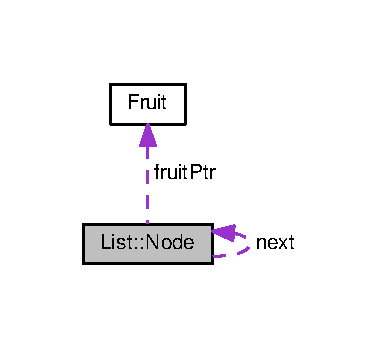
\includegraphics[width=182pt]{structList_1_1Node__coll__graph}
\end{center}
\end{figure}
\subsection*{Public Member Functions}
\begin{DoxyCompactItemize}
\item 
\hyperlink{structList_1_1Node_a3832f8af7db4dc1984446e030144a8cf}{Node} (\hyperlink{classFruit}{Fruit} $\ast$a\+Fruit)
\end{DoxyCompactItemize}
\subsection*{Public Attributes}
\begin{DoxyCompactItemize}
\item 
\hyperlink{classFruit}{Fruit} $\ast$ \hyperlink{structList_1_1Node_a0014e96ae0a971590091f68233a8de2f}{fruit\+Ptr}
\item 
\hyperlink{structList_1_1Node}{Node} $\ast$ \hyperlink{structList_1_1Node_a0e9bd3ca8dc4c1307c04ecb2250fdada}{next}
\end{DoxyCompactItemize}


\subsection{Constructor \& Destructor Documentation}
\index{List\+::\+Node@{List\+::\+Node}!Node@{Node}}
\index{Node@{Node}!List\+::\+Node@{List\+::\+Node}}
\subsubsection[{\texorpdfstring{Node(\+Fruit $\ast$a\+Fruit)}{Node(Fruit *aFruit)}}]{\setlength{\rightskip}{0pt plus 5cm}List\+::\+Node\+::\+Node (
\begin{DoxyParamCaption}
\item[{{\bf Fruit} $\ast$}]{a\+Fruit}
\end{DoxyParamCaption}
)\hspace{0.3cm}{\ttfamily [inline]}}\hypertarget{structList_1_1Node_a3832f8af7db4dc1984446e030144a8cf}{}\label{structList_1_1Node_a3832f8af7db4dc1984446e030144a8cf}

\begin{DoxyCode}
52 \{\hyperlink{structList_1_1Node_a0014e96ae0a971590091f68233a8de2f}{fruitPtr} = aFruit; \hyperlink{structList_1_1Node_a0e9bd3ca8dc4c1307c04ecb2250fdada}{next} = NULL; \}
\end{DoxyCode}


\subsection{Member Data Documentation}
\index{List\+::\+Node@{List\+::\+Node}!fruit\+Ptr@{fruit\+Ptr}}
\index{fruit\+Ptr@{fruit\+Ptr}!List\+::\+Node@{List\+::\+Node}}
\subsubsection[{\texorpdfstring{fruit\+Ptr}{fruitPtr}}]{\setlength{\rightskip}{0pt plus 5cm}{\bf Fruit}$\ast$ List\+::\+Node\+::fruit\+Ptr}\hypertarget{structList_1_1Node_a0014e96ae0a971590091f68233a8de2f}{}\label{structList_1_1Node_a0014e96ae0a971590091f68233a8de2f}
\index{List\+::\+Node@{List\+::\+Node}!next@{next}}
\index{next@{next}!List\+::\+Node@{List\+::\+Node}}
\subsubsection[{\texorpdfstring{next}{next}}]{\setlength{\rightskip}{0pt plus 5cm}{\bf Node}$\ast$ List\+::\+Node\+::next}\hypertarget{structList_1_1Node_a0e9bd3ca8dc4c1307c04ecb2250fdada}{}\label{structList_1_1Node_a0e9bd3ca8dc4c1307c04ecb2250fdada}


The documentation for this struct was generated from the following file\+:\begin{DoxyCompactItemize}
\item 
\hyperlink{Fruit_8cpp}{Fruit.\+cpp}\end{DoxyCompactItemize}

\hypertarget{classOrange}{}\section{Orange Class Reference}
\label{classOrange}\index{Orange@{Orange}}


Inheritance diagram for Orange\+:
\nopagebreak
\begin{figure}[H]
\begin{center}
\leavevmode
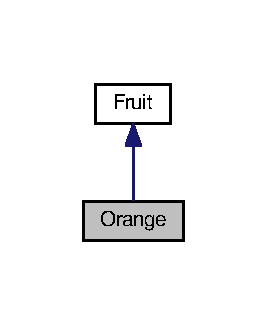
\includegraphics[width=128pt]{classOrange__inherit__graph}
\end{center}
\end{figure}


Collaboration diagram for Orange\+:
\nopagebreak
\begin{figure}[H]
\begin{center}
\leavevmode
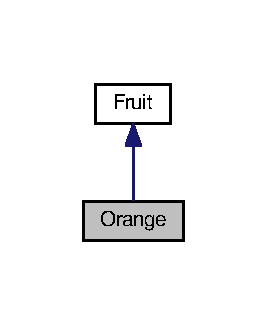
\includegraphics[width=128pt]{classOrange__coll__graph}
\end{center}
\end{figure}
\subsection*{Public Member Functions}
\begin{DoxyCompactItemize}
\item 
\hyperlink{classOrange_ad34fe19e80692b3f206aa22606cf106d}{Orange} (string name, string kind)
\item 
virtual void \hyperlink{classOrange_acb75bbb15104ce63afa0cc6712e239e4}{print} () const 
\end{DoxyCompactItemize}
\subsection*{Private Attributes}
\begin{DoxyCompactItemize}
\item 
string \hyperlink{classOrange_a1bb7a0b91b14b34eafa745fbcd36f325}{thing}
\end{DoxyCompactItemize}
\subsection*{Additional Inherited Members}


\subsection{Constructor \& Destructor Documentation}
\index{Orange@{Orange}!Orange@{Orange}}
\index{Orange@{Orange}!Orange@{Orange}}
\subsubsection[{\texorpdfstring{Orange(string name, string kind)}{Orange(string name, string kind)}}]{\setlength{\rightskip}{0pt plus 5cm}Orange\+::\+Orange (
\begin{DoxyParamCaption}
\item[{string}]{name, }
\item[{string}]{kind}
\end{DoxyParamCaption}
)\hspace{0.3cm}{\ttfamily [inline]}}\hypertarget{classOrange_ad34fe19e80692b3f206aa22606cf106d}{}\label{classOrange_ad34fe19e80692b3f206aa22606cf106d}

\begin{DoxyCode}
37 : \hyperlink{classFruit_ad5e1cedbbe3153aad5b66533f9664e64}{Fruit}(name) \{ \hyperlink{classOrange_a1bb7a0b91b14b34eafa745fbcd36f325}{thing} = kind; \}
\end{DoxyCode}


\subsection{Member Function Documentation}
\index{Orange@{Orange}!print@{print}}
\index{print@{print}!Orange@{Orange}}
\subsubsection[{\texorpdfstring{print() const }{print() const }}]{\setlength{\rightskip}{0pt plus 5cm}virtual void Orange\+::print (
\begin{DoxyParamCaption}
{}
\end{DoxyParamCaption}
) const\hspace{0.3cm}{\ttfamily [inline]}, {\ttfamily [virtual]}}\hypertarget{classOrange_acb75bbb15104ce63afa0cc6712e239e4}{}\label{classOrange_acb75bbb15104ce63afa0cc6712e239e4}


Implements \hyperlink{classFruit_aa939d4077d9be227dde4e8649649c5a2}{Fruit}.


\begin{DoxyCode}
38 \{cout << \hyperlink{classFruit_a97df614e17aebaae352e97d51c801906}{owner} << \textcolor{stringliteral}{"'s orange "} << \hyperlink{classOrange_a1bb7a0b91b14b34eafa745fbcd36f325}{thing} << endl;\}
\end{DoxyCode}


\subsection{Member Data Documentation}
\index{Orange@{Orange}!thing@{thing}}
\index{thing@{thing}!Orange@{Orange}}
\subsubsection[{\texorpdfstring{thing}{thing}}]{\setlength{\rightskip}{0pt plus 5cm}string Orange\+::thing\hspace{0.3cm}{\ttfamily [private]}}\hypertarget{classOrange_a1bb7a0b91b14b34eafa745fbcd36f325}{}\label{classOrange_a1bb7a0b91b14b34eafa745fbcd36f325}


The documentation for this class was generated from the following file\+:\begin{DoxyCompactItemize}
\item 
\hyperlink{Fruit_8cpp}{Fruit.\+cpp}\end{DoxyCompactItemize}

\chapter{File Documentation}
\hypertarget{Fruit_8cpp}{}\section{Fruit.\+cpp File Reference}
\label{Fruit_8cpp}\index{Fruit.\+cpp@{Fruit.\+cpp}}
{\ttfamily \#include $<$string$>$}\\*
{\ttfamily \#include $<$iostream$>$}\\*
Include dependency graph for Fruit.\+cpp\+:
\nopagebreak
\begin{figure}[H]
\begin{center}
\leavevmode
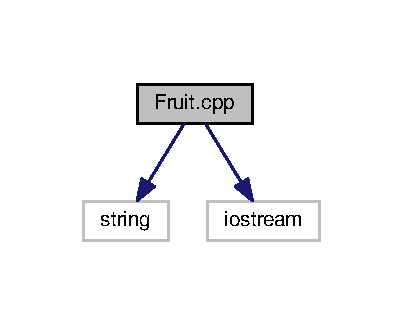
\includegraphics[width=194pt]{Fruit_8cpp__incl}
\end{center}
\end{figure}
\subsection*{Classes}
\begin{DoxyCompactItemize}
\item 
class \hyperlink{classFruit}{Fruit}
\item 
class \hyperlink{classApple}{Apple}
\item 
class \hyperlink{classOrange}{Orange}
\item 
class \hyperlink{classGrape}{Grape}
\item 
class \hyperlink{classList}{List}
\item 
struct \hyperlink{structList_1_1Node}{List\+::\+Node}
\end{DoxyCompactItemize}
\subsection*{Functions}
\begin{DoxyCompactItemize}
\item 
int \hyperlink{Fruit_8cpp_ae66f6b31b5ad750f1fe042a706a4e3d4}{main} ()
\end{DoxyCompactItemize}


\subsection{Function Documentation}
\index{Fruit.\+cpp@{Fruit.\+cpp}!main@{main}}
\index{main@{main}!Fruit.\+cpp@{Fruit.\+cpp}}
\subsubsection[{\texorpdfstring{main()}{main()}}]{\setlength{\rightskip}{0pt plus 5cm}int main (
\begin{DoxyParamCaption}
{}
\end{DoxyParamCaption}
)}\hypertarget{Fruit_8cpp_ae66f6b31b5ad750f1fe042a706a4e3d4}{}\label{Fruit_8cpp_ae66f6b31b5ad750f1fe042a706a4e3d4}

\begin{DoxyCode}
83            \{
84     \textcolor{comment}{// the Apple pointer is cast to a Fruit pointer in the List constructor}
85     \hyperlink{classList}{List} myList(\textcolor{keyword}{new} \hyperlink{classApple}{Apple}(\textcolor{stringliteral}{"Tom"}));
86 
87     \textcolor{comment}{// similarly the Grape and Orange pointers are cast to Fruit* in append}
88     myList.append(\textcolor{keyword}{new} \hyperlink{classGrape}{Grape}(\textcolor{stringliteral}{"Steve"}));
89     myList.append(\textcolor{keyword}{new} \hyperlink{classOrange}{Orange}(\textcolor{stringliteral}{"Lori"},\textcolor{stringliteral}{"juice"}));
90     myList.printList(); 
91     cout << endl;
92     \textcolor{keywordflow}{return} 0;
93 \}
\end{DoxyCode}


Here is the call graph for this function\+:
\nopagebreak
\begin{figure}[H]
\begin{center}
\leavevmode
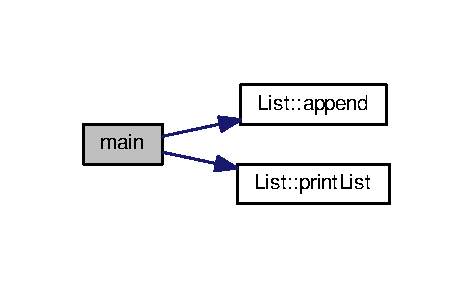
\includegraphics[width=227pt]{Fruit_8cpp_ae66f6b31b5ad750f1fe042a706a4e3d4_cgraph}
\end{center}
\end{figure}



%--- End generated contents ---

% Index
\backmatter
\newpage
\phantomsection
\clearemptydoublepage
\addcontentsline{toc}{chapter}{Index}
\printindex

\end{document}
